\documentclass[xcolor=dvipsnames,10pt]{beamer}

\usepackage[utf8]{inputenc}
\usepackage[spanish]{babel}
\usepackage{multirow,rotating}
\usepackage{amsfonts,amsmath,amssymb,amsthm}
\usepackage{color}
\usepackage{hyperref}
\usepackage{fourier,libertine}
\usepackage{transparent}
\usepackage{tikz-cd}
\usepackage{array}
\usepackage{algpseudocode}
\usepackage{siunitx}
\usepackage{algorithm}
\usepackage{mathtools,nccmath}%
\usetheme{Madrid}
\usepackage{xcolor}
\usepackage{natbib}
\usepackage{hyperref}
\usepackage{ragged2e}
\usefonttheme{serif}
\usefonttheme{professionalfonts}
\newcommand\T{\ensuremath{\mathbb{T}}}
\newcommand\N{\ensuremath{\mathbb{N}}}
\newcommand\R{\ensuremath{\mathbb{R}}}
\newcommand\Z{\ensuremath{\mathbb{Z}}}
\renewcommand\O{\ensuremath{\emptyset}}
\newcommand\Q{\ensuremath{\mathbb{Q}}}
\newcommand\C{\ensuremath{\mathbb{C}}}
\newcommand\Hs{\ensuremath{\mathbb{H}}}
% set color ------------------------------------------------------------------
\definecolor{DarkBlue}{rgb}{0.04706, 0.13725, 0.26667} 
\definecolor{cadmiumred}{rgb}{0.45 , 0.12, 0.23}
\definecolor{armygreen}{rgb}{0.10, 0.27, 0.19}
\definecolor{coolblack}{rgb}{0.0, 0.18, 0.39}
\definecolor{lilac}{rgb}{0.33, 0.12, 0.36}
\definecolor{negro}{rgb}{0, 0, 0}
\usecolortheme[named=coolblack]{structure}
\setbeamercolor{block title}{bg=coolblack!100!white,fg=white}
\setbeamercolor{block body}{bg=coolblack!11!white}

%----------------------------------------------------------------------------
\setbeamerfont{title}{size=\large}
\setbeamerfont{subtitle}{size=\small}
\setbeamerfont{author}{size=\small}
\setbeamerfont{date}{size=\footnotesize}
\setbeamerfont{institute}{size=\footnotesize}
\title[Universidad Nacional de Colombia]{Espacios de Teichmuller y Moduli}
\subtitle{Universidad  Nacional de Colombia.}
\author[Superficies de Riemann]{Sergio Alejandro Bello Torres\\
Edgar Santiago Ochoa Quiroga}

\date[\textcolor{white}{Julio/2025}]


\begin{document}
\maketitle
\begin{frame}{Introducción}
    Uno de los problemas principales en el estudio de las superficies de Riemann es su clasificación, en particular hemos visto que una misma superficie puede tener dos estructuras complejas completamente diferentes, por lo que nos interesamos en caracterizar todas estas estructuras. A partir de este problema surgen los espacios de Moduli y Teichmüller, que por su estructura ayudan a clasificar todas las posibles estructuras complejas de una superficie dada. Nuestro propósito es hacer una breve introducción a éstos espacios, incluyendo algunas construcciones elementales.

\end{frame}
\begin{frame}{Preliminares Topología Algebraica}

    \begin{block}{Definición}
        Dos caminos $\gamma_1$ y $\gamma_2$ que envian el intervalo $[0,1]$ en un espacio topológico $X$, se dice que son \textbf{caminos homotopicos} si ambos tienen el mismo punto inicial $x_0$ y final $x_1$, y además existe una funcion continua $F:[0,1]\times[0,1]\to X$ tal que
        $$F(s,t)=\begin{cases}
        \gamma_1(s) & Si\,t=0,\\
        \gamma_2(s) & Si\,t=1,\\
        x_0& Si\,s=0,\\
        x_1& Si\,s=1.
        \end{cases}$$
        \end{block}
        \begin{figure}
        \centering
        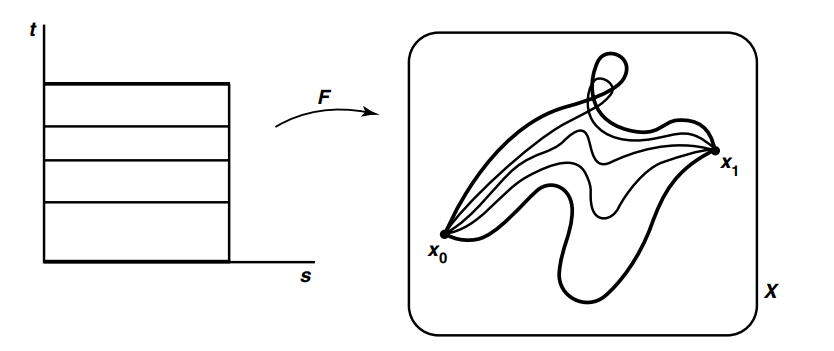
\includegraphics[width=0.5\linewidth]{Imagenes/imagen_2025-07-10_112455145.png}
    \end{figure}
\end{frame}
\begin{frame}
    \begin{block}{Definición}
        Dado $X$ espacio topológico y $x_0\in X$. El conjunto de clases de homotopía de caminos cuyo punto inicial y final es $x_0$, junto a la operacion de concatenar caminos lo llamamos el \textbf{grupo fundamental} de $X$ relativo a $x_0$ y que denotaremos por $\pi_1(X,x_0)$
        \end{block}

        \begin{block}{Definición}
        Un espacio topológico $X$ se dice \textbf{simplemente conexo} si es arco-conexo y su grupo fundamental es el trivial.
        \end{block}  
        \begin{block}{Definición}
            Sean $X,Y$ espacios topológicos y $h: X \rightarrow Y$ una función contínua tal que $f(x_0) = y_0$, definimos $h_*:\pi_1(X,x_0)\rightarrow \pi_1(Y,y_0)$, tal que $h_*([f]) = [(h \circ f)]$. Llamamos a $h_*$ el \textbf{homomorfismo inducido} por $h$.
        \end{block}
\end{frame}
\begin{frame}
    \begin{block}{Definición}
        Sea $p:E\to B$ una función contínua y sobreyectiva. Dado un abierto $U$ de $B$ se dice que esta cubierto uniformemente por $p$ is la imagen inversa de $U$ por $p$ puede ser escrita como unión de abiertos disyuntos $V_\alpha$ en $E$, y la restricción de $p$ a cada uno de estos es un homeomorfismo.
        \end{block} 
        \begin{figure}
            \centering
            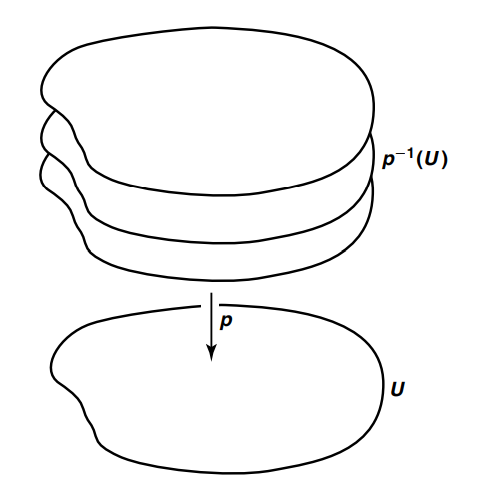
\includegraphics[width=0.4\linewidth]{Imagenes/imagen_2025-07-10_120527033.png}
        \end{figure}   
\end{frame}
\begin{frame}
        \begin{block}{Definición}
        Si para cada punto $b$ existe una vecindad $U$ tal que ésta esté cubierta uniformemente se dice que $p$ es una funcion recubridora y que $E$ es un \textbf{espacio recubridor}
        \end{block} 
        \begin{block}{Definición}
            Si el espacio recubridor $E$ es simplemente conexo se le llama el \textbf{cubrimiento universal}.
        \end{block}
        Al referirnos al cubrimiento universal de un espacio $X$ lo denotaremos por $\tilde{X}.$
        
\end{frame}
\begin{frame}{Teorema de Uniformizacion}
    \begin{block}{Teorema}
        Sea $X$ una superficie de Riemann simplemente conexa, entonces $X$ es biholomorfa a exactamente una de las siguientes superficies
        \begin{itemize}
            \item La esfera de Riemann $\C_{\infty}.$
            \item El plano Complejo $\C.$
            \item El semiplano superior $\Hs^2.$
        \end{itemize}
    \end{block}
    \textbf{Observación:} Note que a el cubrimiento universal lo podemos dotar de una estructura de superficie Riemann a partir de la de $X$, por lo que podemos pensar a las superficies de Riemann como cocientes de su cubrimiento universal.  
\end{frame}
\begin{frame}{Cocientes de superficies}
    En vista de lo anterior, lo natural seria pensar en las superficies de Riemann simplemente conexas y ver su posibles cocientes, pero resulta que para la esfera de Riemann y el plano complejo tenemos poca variedad
    \begin{block}{Proposicion}
        Sea $X$ una superficie de Riemann. El cubrimiento universal de $X$ es biholomorfo a $\C_\infty$ si y solo si $X$ es biholomorfo a $\C_\infty$
    \end{block}
    \begin{block}{Proposicion}
        Sea $X$ una superficie de Riemann. El cubrimiento universal de $X$ es biholomorfo a $\C$ si y solo si $X$ es biholomorfo a $\C,\C-\{0\}$ o $\C/L$
    \end{block}
    Resulta que donde tendremos una mayor variedad son los cocientes de $\Hs^2$.
\end{frame}
\begin{frame}{Superficies Hiperbólicas}

Los cocientes de $\Hs^2$ son lo que denominaremos como superficies hiperbólicas. Se tiene que $\Hs^2$ viene equipado con una métrica dada por
$$ds^2=\dfrac{dx^2+dy^2}{y^2},$$
ademas el grupo de automorfismos $PSL(2,\R)$ de $\Hs^2$, es justamente el grupo de isometrias que preservan la orientación de esta métrica.\\
\vspace{0.3cm}
\textbf{Observación:} Todos los cocientes de $\Hs^2$ que dan lugar a una superficie de Riemann heredan una métrica completa de curvatura constante $-1$, es decir una métrica hiperbólica. Mas aun toda métrica de la que se puede dotar una superficie da lugar a una superficie de Riemann.
    
\end{frame}
\begin{frame}{Espacio de Teichmuller del Toro}
    En general un espacio de Teichmüller asociado a una superficie sera el espacio de superficies de Riemann \textit{marcadas} de aquella superficie, mientras que el espacio de Moduli sera el de clases de isomorfismo de estas estructuras.\\
    \vspace{0.5cm}

    Por el Teorema de Uniformizacion solo podemos asignarle una estructura de superficie de Riemann a $\C_\infty$, por lo que segun nuestra idea general el espacio de Moduli es un único punto. Resulta que para el espacio de Teichmuller ocurre lo mismo, por lo que nuestro interés inicial sera estudiar estos espacios para los toros $\C/L$
\end{frame}
\begin{frame}
    Recordemos que los retículos están determinados por una base de la forma $\{1,\tau\}$, donde $\tau\in \Hs^2$, por lo cual cualquier estructura compleja del toro viene determinada por un punto del plano hiperbólico. Sin embargo pueden existir $\tau, \tau' \in \Hs^2$ con $\tau \neq \tau'$ que resulten en dos estructuras biholomorfas.

    \begin{block}{Proposición}
        Sean $\C/L$ y $\C/L'$ dos toros determinados por $\tau$ y $\tau'$ respectivamente, entonces son biholomorfos si y solo si
        \[
            \tau' = \frac{a\tau + b}{c\tau + d}
        \]
        Con $a,b,c,d \in \Z$ y $ad-bc=1$
    \end{block}

    Esto quiere decir que las estructuras de superficie de Riemann del toro están determinadas por la acción de $\text{SL}(2,\Z)$ sobre $\Hs^2$
\end{frame}
\begin{frame}
    Sea $\mathcal{M}_1 = \Hs^2/\text{SL}(2,\Z) = \Hs^2/\text{PSL}(2,\Z)$ queremos ver como es la topología de este cociente. 
    \begin{block}{Definición}
        Sea $G$ un grupo y $X$ espacio topologico. Si $G$ actua sobre $X$ definimos un dominio fundamental como un subespacio de $X$ cerrado tal que su interior contiene solo un elemento de cada orbita.
    \end{block}
    Con esta idea podemos estudiar la estructura del cociente presentado. Considere el conjunto 
    $$\mathcal{F}=\left\{z\in\Hs^2:|z|\geq 1\text{ y } |Re(z)|\leq \frac{1}{2}\right\}.$$
    \begin{figure}
            \centering
            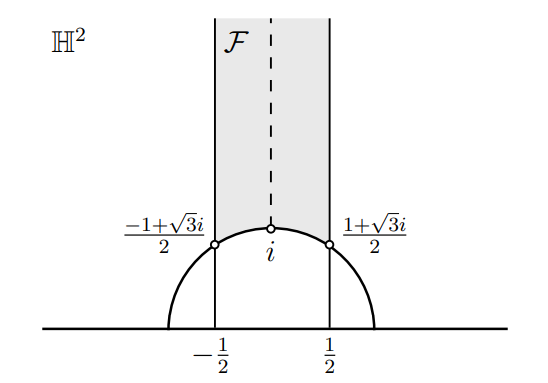
\includegraphics[width=0.4\linewidth]{Imagenes/FunDom.png}
        \end{figure} 
    
\end{frame}
\begin{frame}
    Note que dado $\tau\in\Hs^2$ existe $g\in PSL(2,\Z)$ tal que $g\tau\in\mathcal{F}.$ Esto se tiene ya que dado tal $g$ un calculo nos muestra que
    $$Im(gz)=\frac{Im(z)}{|cz+d|^2},$$
    Podemos tomar $g$ tal que $Im(g\tau)$ es maximal y de hecho es maximo. Luego podemos trasladar por medio de $z\to z+1$ hasta que $|Re(g\tau)|\leq \dfrac{1}{2}.$ Si $|g\tau|<1$ entonces $\left|\dfrac{1}{g\tau}\right|>1$ y eso contradice la maximalidad de la parte imaginaria.\\
    Podemos ver que
    \begin{itemize}
        \item Si $\tau\in Int(\mathcal{F})$ entonces $O(\tau)\cap\mathcal{F}=\{\tau\}.$ 
        \item Si $Re(\tau)=\pm\dfrac{1}{2}$ entonces $O(\tau)\cap\mathcal{F}=\{\tau,\tau\mp1\}.$
        \item Si $|\tau|=1$ entonces $O(\tau)\cap \mathcal{F}=\left\{\tau,-\dfrac{1}{\tau}\right\}.$
    \end{itemize}
    
\end{frame}
\begin{frame}
    Asumamos que $z,gz\in\mathcal{F}$, luego asuma que $Im(gz)\geq Im(z)$, así $|cz+d|\leq 1,$ por la relación de antes. Como $|z|\geq 1$, tenemos que $c=\pm1,0.$\\

    Si $c=0$, $d=\pm 1$ y por la condición sobre el determinante $gz=z+b$, luego $b=0,\pm 1$, si $b=0$ ya tenemos el primer caso. En cambio si $b=\mp 1$, tenemos que $Re(z)=\pm\dfrac{1}{2}.$\\

    Por ultimo si $c=\pm 1$, forzosamente $d=0$ y $|z|=1$, asi $gz=-\dfrac{1}{z}.$\\

    Concluimos que $\mathcal{M}_1$ es el espacio que resulta de identificar los bordes de $\mathcal{F}$
    \begin{figure}
            \centering
            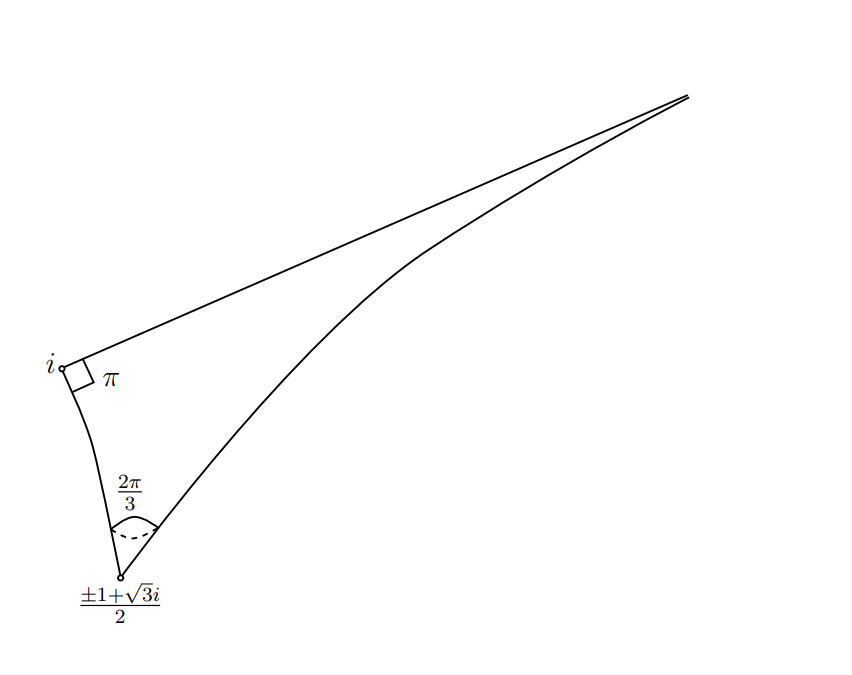
\includegraphics[width=0.5\linewidth]{Imagenes/Empanada.png}
        \end{figure} 

    $\mathcal{M}_1$ se denomina el espacio de móduli del toro y $\mathcal{T}_1 = \Hs^2 $ es el espacio de Teichmüller
\end{frame}
\begin{frame}
    Habiendo hecho esto, queremos generalizar éstos espacios a superficies de género más alto, vimos que fue sencillo construir los espacios de Teichmüller y móduli del toro debido a una particularidad muy especial, sin embargo, éstas particularidades pueden ser entendidas de otra manera, si tomamos $p_0 = [0] \in \C /L$, podemos ver que los segmentos $\overline{[0:1]}$ y $\overline{[0:\tau]}$ del plano complejo tienen asociados dos caminos cerrados que determinan dos generadores $[A_\tau],[B_\tau]$ de $\pi_1(\C /L,p_0)$, si además, tenemos $f: \C/L \rightarrow \C/L'$ un biholorfismo, el homomorfismo inducido $f_*: \pi_1(\C/L,p_0) \rightarrow \pi_1(\C/L', p_0)$ no necesariamente envía $[A_\tau],[B_\tau]$ a $[A_{\tau'}],[B_{\tau'}]$, de hecho ésto solo ocurre si $\tau = \tau'$. Ésta idea será la que nos ayudará a conseguir nuestro objetivo principal.
    \begin{figure}
            \centering
            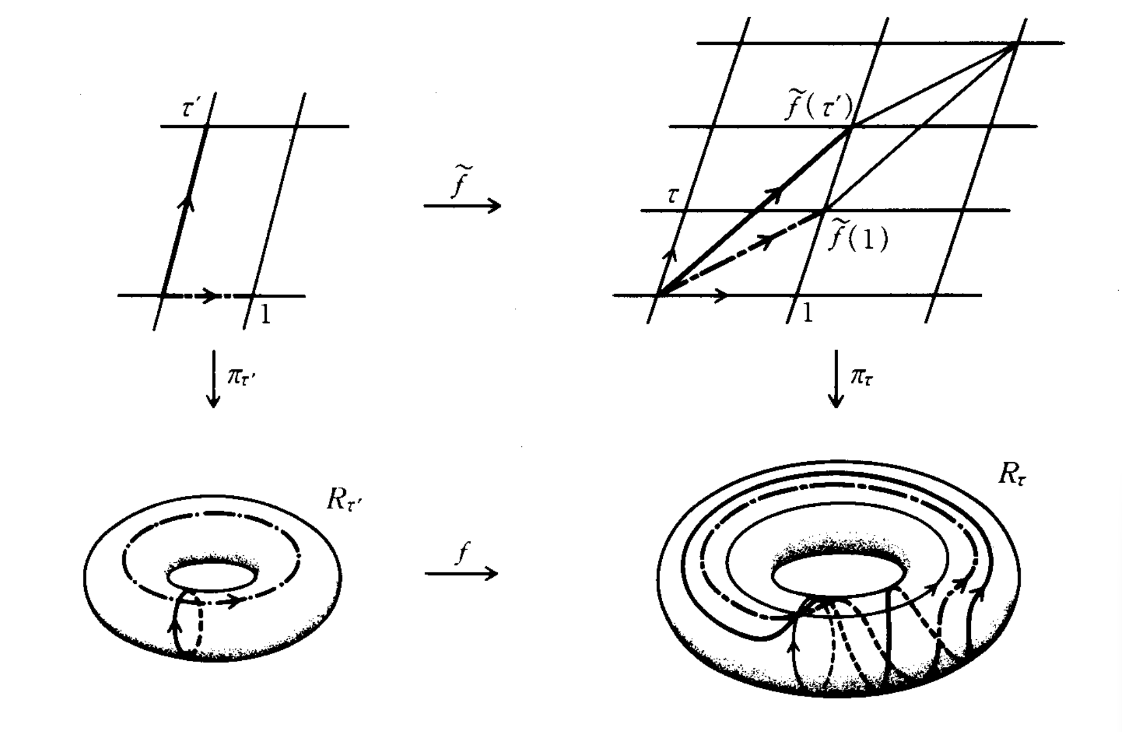
\includegraphics[width=0.5\linewidth]{Imagenes/Marking.png}
        \end{figure}  
\end{frame}
\begin{frame}{Marking}
    \begin{block}{Definición}
        Sea $X$ una superficie de Riemann cerrada género g,  decimos que $\Sigma_g = \{[A_1],[A_2],\ldots,[A_g],[B_1],[B_2],\ldots, [B_g]\}$ es un \textbf{sistema canónico de generadores} para $\pi_1(X,p_0)$ si
    \[ \prod_{i=1}^g [A_i,B_i] = e \]
    \begin{itemize}
        \item Un \textit{marking} en $X$ es un sistema canónico de generadores $\Sigma_p \subset \pi_1(X,p)$
        \item Dos markings $\Sigma_p$ y $\Sigma_{p'}^\prime$ se dicen  \textbf{equivalentes} si existe una curva contínua $\alpha$ entre $p$ y $p'$, tal que el isomorfismo inducido $T_\alpha: \pi_1(X,p) \rightarrow \pi_1(X,p')$ satisface
        \[
        T_\alpha(\Sigma_p) = \Sigma_p'
        \]
    \end{itemize}
    Al par $(X,\Sigma_p)$ lo llamamos \textbf{superficie de Riemann marcada} 
    \end{block}
    \end{frame}

    \begin{frame}
        Entonces siguiendo la construcción hecha para el Toro el espacio de Teichmuller de una superficie $X$ cerrada, es el conjunto de las superficies marcadas que son difeomorfas a $X$ modulo equivalencia.\\
        \vspace{0.3cm}
        Con esto tenemos una caracterización del espacio de Teichmuller, pero no nos da información sobre su topología, asi es como introducimos el \textit{Marking por difeomorfismos.} 
    \end{frame}
    \begin{frame}
        \begin{block}{Definición}
            Sean $R$ y $R^\prime$ superficies de Riemann, definamos
            \begin{align*}
                 f:X\to R\,\text{  y  }\,f^\prime:X\to R^\prime,
             \end{align*} 
             como difeomorfismos que preservan la orientación. Decimos que las parejas $(R,f)$ y $(R^\prime,f^\prime)$ son equivalentes si existe un biholomorfismo $h:R\to R^\prime$ tal que
             $$(f^\prime)^{-1}\circ h\circ f:X\to X,$$
             es homotopico a la identidad.
        \end{block}
        \textbf{Observación:} Si escogemos un conjunto de generadores $\Sigma$ para el grupo fundamental $\pi_1(X,p)$, entonces cada pareja $(R,f)$ define un punto
        $$(R,f_{*}(\Sigma))\in \mathcal{T}.$$
        Donde $\mathcal{T}$ es el espacio de Teichmuller de $X.$
        
    \end{frame}
    \begin{frame}
        La definición anterior nos brinda una nueva descripción del espacio de Teichmuller de una superficie $X.$
        $$\mathcal{T}(X)=\left\{(R, f): \begin{array}{c}R \text{ es una superficie de Riemann }, f: X \rightarrow R \\ \text{ un difeomorfismo que preserva la orientación }\end{array}\right\} / \sim.$$
        Con esta nueva descripción sera mucho mas sencillo describir el espacio de Moduli, con lo que llamaremos \textit{Mapping class group.}
    \end{frame}

    \begin{frame}{Mapping class group}
        Sea $X$ una superficie de Riemann cerrada. Definimos
        $$Diff^+(X)=\left\{f:X\to X| f \text{ es un difeomorfismo que preserva la orientación }\right\},$$
        y
        $$Diff^+_0(X)=\left\{f\in Diff^+(X):f\text{ es homotopico a la identidad}\right\}.$$
        Podemos notar que $Diff^+(X)$ es un grupo y que $Diff^+_0(X)$ es un subgrupo normal de $Diff^+(X).$ Con lo cual 
        \begin{block}{Definición}
            El \textbf{Mapping class group} de una superficie de riemann cerrada $X$ es
            $$MCG(X):=Diff^+(X)/Diff^+_0(X).$$
        \end{block}
        
    \end{frame}
    \begin{frame}{Espacio de Moduli}
        El \textit{Mappin class group} actua sobre el espacio de Teichmuller de la siguiente manera:
        $$[g]\cdot[(R,f)]=[(R,f\circ g^{-1})].$$
        El cociente de el espacio de Teicchmuller por esta acción es lo que llamaremos espacio de Moduli, es decir
        \begin{block}{Definición}
            El \textbf{espacio de Moduli} de una superficie de Riemann cerrada $X$ es
            $$\mathcal{M}(X)=\mathcal{T}(X)/MCG(X).$$
        \end{block}
        Si $X$ es una superficie cerrada de genero $g$, se suele denotar $\mathcal{T}(X)=\mathcal{T}_g$ y $\mathcal{M}(X)=\mathcal{M}_g$
    \end{frame}
    \begin{frame}
        Ya hemos construido los espacios de Teichmuller y Moduli para las superficies cerradas de genero $g$. Sabemos que estos espacios nos dan información sobre las estructuras complejas de estas superficies, pero ahora queremos saber que relación guarda una estructura con otra. De estudiar este problema es donde aparecen las \textbf{aplicaciones cuasiconformes}.
    \end{frame}

    

\begin{frame}{Aplicaciones conformes y cuasiconformes}
Sea $w=f(z)$ un homeomorfismo $C^1$ de una región a otra. En un punto $z_0$ se inducen aplicaciones lineales de diferenciales tal que
\begin{align*}
    du&=u_xdx+u_ydy,\\
    dv&=v_xdx+v_ydy.\\
\end{align*}
Estos también se pueden ver de manera compleja como
$$dw=f_zdz+f_{\overline{z}}d\overline{z},$$
donde $z=x+iy$ y $w=u+iv.$ Geometricamente  estos representan transformaciones afines del plano $(dx,dy)$ al plano
$(du,dv).$\\

De esta manera estas transformaciones envían círculos centrados en el origen en elipses similares, es de nuestro interés ver la razón entre los ejes y como cambia su dirección.    

\end{frame}

\begin{frame}
    Observemos ahora si que podemos escribir
    \begin{align*}
        f_z&=\frac{1}{2}(u_x+u_y)+\frac{i}{2}(v_x-u_y),\\
        f_{\overline{z}}&=\frac{1}{2}(u_x-v_y)+\frac{i}{2}(v_x+u_y).
    \end{align*}
    Con esto podemos notamos
    $$|f_z|^2-|f_{\overline{z}}|^2=u_xv_y-u_yv_x=J.$$
    Donde $J$ es el Jacobiano de la transformación. Como solo estamos considerando las aplicaciones que preservan la orientación, el Jacobiano es positivo, luego $|f_{\overline{z}}|<|f_z|$, de esto se sigue que
    $$(|f_z|-|f_{\overline{z}}|)|dz|\leq |dw|\leq (|f_z|+|f_{\overline{z}}|)|dz|.$$
    Donde ambos extremos de la desigualdad se alcanzan, asi obtenemos que la razon esta dada por
    $$D_f=\frac{|f_z|+|f_{\overline{z}}|}{|f_z|-|f_{\overline{z}}|}\geq 1.$$
    Esto se conoce como la \textbf{dilatación} en el punto $z$.
\end{frame}

\begin{frame}
    \begin{block}{Definición}
        La aplicación $f$ se dice \textbf{cuasiconforme} si $D_f$ es acotada.
        \end{block}
        Particularmente obtenemos que
\begin{block}{Proposición}
Si $D_f=1$ tenemos que $f$ es una aplicación \textbf{conforme}.
\end{block}
Resulta mas conveniente considerar
    $$d_f=\frac{|f_{\overline{z}}|}{|f_z|}<1,$$
    que se relaciona con $D_f$ tal que
    $$D_f=\frac{1+d_f}{1-d_f}.$$
\end{frame}
\begin{frame}
    \begin{block}{Definición}
        La \text{dilatación compleja} esta dada por
        $$\mu_f=\frac{f_{\overline{z}}}{f_z}.$$
        LLamamos a $\mu_f$ el \textit{coeficiente de Beltrami de }$f.$
    \end{block}
    \begin{figure}
            \centering
            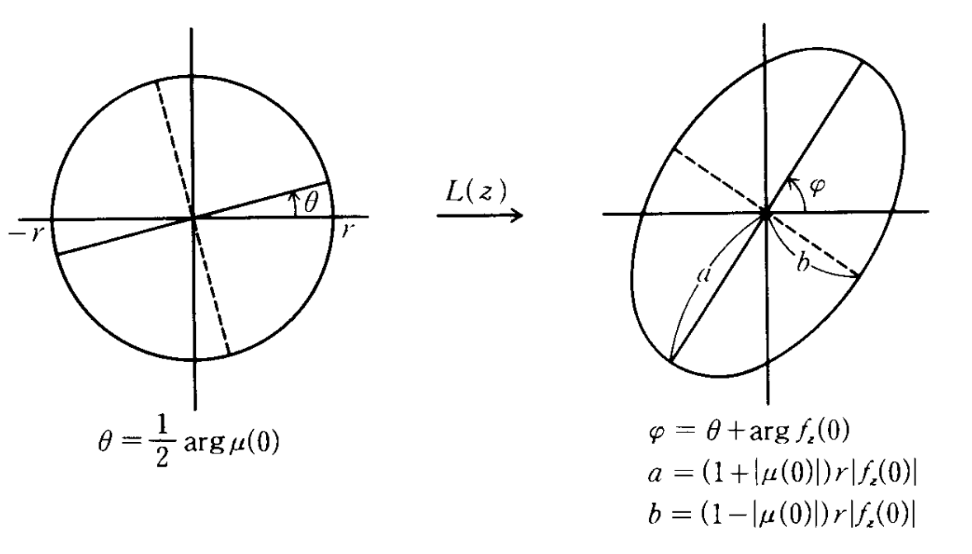
\includegraphics[width=0.5\linewidth]{Imagenes/Semieje.png}
        \end{figure}
\end{frame}

\begin{frame}{Relacion con el espacio de Teichmuller}
    Consideremos $[(R,f)]\in\mathcal{T}(X)$, es de nuestro interes comparar la estructura compleja de $R$ y $X$, para esto tomamos una vecindad $U$ y una coordenada local $z$ en $R$, de manera similar $V$ vecindad y $w$ coordenada local en $X.$ Si consideramos $F=w\circ f\circ z^{-1}$ entonces 
    $$\mu_F=\frac{F_{\overline{z}}}{F_z},$$
    es una función suave de valor complejo y ademas no depende de la coordenada local $w.$ Además $\mu_F$ cumple todas las condiciones de un coeficiente de Beltrami.
\end{frame}
\begin{frame}
    Si $\{(U_\alpha,w_\alpha)\}$ es un atlas en $X$ y $f:R\rightarrow X$ es un difeomorfismo que preserva la orientación, la colección $\{(f^{-1}(V_\alpha),w_\alpha \circ f)\}$ es tambien un atlas en $R$. En este sentido tenemos una nueva superficie de Riemann $R_f$ con el sistema de coordenadas dado previamente.\\
    \vspace{0.3cm}
    Podemos notar que la función identidad de $R$ a $R_f$ es un difeomorfismo que preserva la orientación. Luego tomando $f:R_f\to X$, este es un biholomorfismo, por lo que $(X,f)=(R_f,id),$ entonces el coeficiente de Beltrami $\mu_F$ nos dice que tanto hay que deformar una superficie en otra para obtener su estructura compleja. Asi podemos construir el espacio de Teichmuller a partir de los coeficientes de Beltrami.
\end{frame}
\begin{frame}{Espacios de coeficientes de Beltrami}

    \begin{block}{Proposición}
        Dadas superficies de Riemann $R,S,T,$ y difeomorfismos que preservan la orientación $f:R\to S$ y $g:S\to T$, se tiene la siguiente relación
        $$\mu_g\circ f=\frac{f_z}{\overline{f_z}}\frac{\mu_{g\circ f}-\mu_f}{1-\overline{\mu_f}\cdot\mu_{g\circ f}}.$$ 
        Es particular si tenemos difeomorfismos que preservan la orientación $f_1:R\to S_1$ y $f_2:R\to S_2$, la aplicacion $f_2\circ f_1^{-1}$ es biholomorfa si y solo si $\mu_{f_1}=\mu_{f_2}.$
    \end{block}
    Ahora construiremos el espacio de Teichmuller en terminos de los coeficientes de Beltrami de $X.$ Sea $B(X)_1$ el conjunto de los coeficientes de Beltrami de $X$, si equipamos a este conjunto con la norma $L^\infty$, hemos una definido una topología. 
\end{frame}
\begin{frame}
    Consideramos la acción de $Diff^+(X)$ sobre $B(X)_1$, dada por
    $$w^*(\mu_f)=\mu_{f\circ w^{-1}}=\left(\frac{w_z}{\overline{w_z}}\frac{\mu_f-\mu_w}{1-\overline{\mu_w}\mu_f}\right)\circ w^{-1},$$
    \begin{block}{Teorema}
        Dados difeomorfismos que preservan la orientación $f:X\to R$ y $g:X\to R^\prime$, existe una aplicacion biholomorfa $h:R\to R^\prime$ si y solo si existe $w\in Diff^+(X)$ tal que $\mu_g=w^*(\mu_f).$ Ademas $g^{-1}\circ h\circ f$ es homotopico a la identidad en $X$ si y solo si $w\in Diff_0^+(X).$ 
    \end{block}
    Esta relación nos dice como son las orbitas del cociente.
    \begin{block}{Corolario}
        La aplicación que envia $(R,f)$ a $\mu_f\in B(X)_1$ induce las siguientes identificaciones
        \begin{align*}
           \mathcal{T}(X)&\cong B(X)_1/Diff_0^+(X),\\
           \mathcal{M}(X)&\cong B(X)_1/Diff^+(X). 
        \end{align*}
    \end{block}
    Con esto hemos inducido una topología, que resulta independiente de la estructura compleja inicial de $X.$
\end{frame}
\begin{frame}{La métrica de Teichmuller}
\begin{block}{Definición}
    Sea $X$ una superficie de Riemann, entonces podemos definir una metrica sobre $\mathcal{T}(X)$ de la siguiente manera
    $$d_T((R_1,f_1),(R_2,f_2))=\frac{1}{2}\log\left(\inf\left\{D_g:\begin{array}{c} g:R_1\to R_2 \text{ es un difeomorfismo que}\\\text{ preserva la orientación homotopico a}\\f_2\circ f_1^{-1}\end{array}\right\}\right).$$
\end{block}
Se puede observar que esta métrica resulta compatible con la topología dada anteriormente.\\

Esta metrica resulta ser una generalizacion de lo que se conoce como \textit{el problema de Grotschz}.
    
\end{frame}

\begin{frame}{Problema de Grotschz}
    Sean $R,R^\prime$ dos rectángulos de lados $a,b$ y $a^\prime,b^\prime$ respectivamente. Queremos ver cual es la aplicación $f$ que enviá $R\to R^\prime$, que sea lo mas conforme posible, con conforme nos referimos a que la norma de la dilatación $D_f$ sea mínima.
    \begin{block}{Teorema}
        Sea 
        $$f(z)=\frac{1}{2}\left(\frac{a^\prime}{a}+\frac{b^\prime}{b}\right)z+\frac{1}{2}\left(\frac{a^\prime}{a}-\frac{b^\prime}{b}\right)\overline{z},$$
        entonces $f(z)$ es solución para el problema de Grotschz.
    \end{block}
    Note que esta funcion representa una transformacion afin que es 
    $$f(x,y)=\left(\frac{a^\prime}{a}x,\frac{b^\prime}{b}y\right).$$
\end{frame}

\begin{frame}{Referencias}
\begin{thebibliography}{9}

\bibitem{ahlfors}
L. V. Ahlfors, \textit{Lectures on Quasiconformal Mappings}, D. Van Nostrand Company, 1966.

\bibitem{petri}
B. Petri, \textit{Introduction to Teichmüller Theory. Lecture Notes}, 2024. disponible \href{https://webusers.imj-prg.fr/~bram.petri/teaching_tt_2425.html}{\textcolor{blue}{aquí}}

\bibitem{Imayoshi}
Y. Imayoshi, M. Taniguchi, \textit{An Introduction to Teichmüller Spaces}, Springer, 1992.

\bibitem{Munkres}
J. Munkres, \textit{Topology}, Pearson, 2014.

\bibitem{abikoff}
W. Abikoff, \textit{The Real Analytic Theory of Teichmüller Space}, Springer, 1980.

\bibitem{hubbard}
J. H. Hubbard, \textit{Teichmüller Theory and Applications to Geometry, Topology and Dynamics}, Vol. 1, Matrix Editions, 2006.


\end{thebibliography}


\end{frame}

\end{document}




